\chapter{Instrukcja wdrożenia}
\label{ch:instrukcja-wdrozenia}

\section{Rozgrywka na platformie Lichess}
\label{sec:rozgrywka-na-platformie-lichess}
Najłatwiejszym i najszybszym sposobem na zmierzenie się z silnikiem jest rozgrywka na platformie lichess.com, do czego autor niniejszej pracy serdecznie zaprasza.
Należy odszukać silnik po nazwie użytkownika \textit{KobayashiMaruPL} i gdy ten będzie aktywny zaprosić go~do~pojedynku.

W celu implementacji tego rozwiązania została wykorzystana biblioteka lichess-bot, która stanowi pośrednik pomiędzy silnikami wykorzystującymi UCI a API platformy Lichess. \cite{lichess-bot-docs}

\section{Kompilacja kodu i połączenie z GUI}
\label{sec:kompilacja-kodu-i-polaczenie-z-gui}

Aby własnoręcznie skompilować kod źródłowy silnika, należy wykonać poniższe kroki:
\begin{enumerate}
    \item Pobrać kod źródłowy z publicznie dostępnego repozytorium \url{https://github.com/KaWis17/KobayashiMaru}.
    \item Stworzyć plik \texttt{.jar} z kodem źródłowym, korzystając z dowolnego narzędzia do~budowania projektów w języku Java.
    \item Stworzyć skrypt \texttt{.sh} zawierający komendę uruchamiającą silnik, np.:~\texttt{java~-jar~KobayashiMaru.jar}.
    \item Sprawdzić poprawność przez odpalenie silnika w konsoli.
    Po wpisaniu na standardowe wejście \texttt{uci} silnik powinien odpowiedzieć zgodnie z protokołem.
    \item Połączyć z interfejsem graficznym według instrukcji dostarczonej przez producenta oprogramowania.
    Dla przykładu w programie CuteChess należy wejść w preferencje ->~silniki -> dodaj silnik -> wybrać skrypt \texttt{.sh} jako komendę.
    \item Rozpocząć grę z silnikiem przez stworzenie nowego meczu.
\end{enumerate}

\begin{figure}[ht]
    \centering
    \begin{tabular}{@{}ll@{}}
        a) & b) \\
        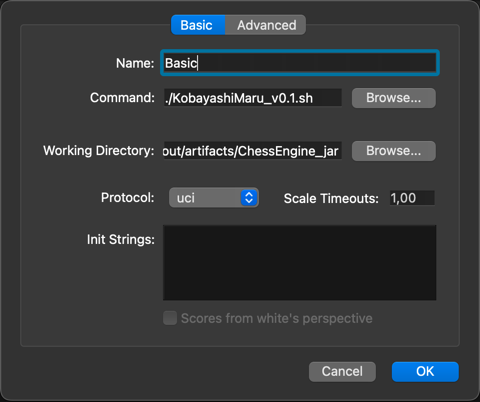
\includegraphics[width=0.25\textwidth]{dodatki/dodatekA/rysunki/instrukcja}
        &
        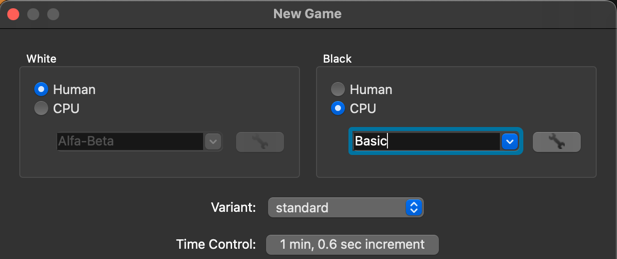
\includegraphics[width=0.5\textwidth]{dodatki/dodatekA/rysunki/nowa-gra}
    \end{tabular}
    \caption{Interfejs graficzny CuteChess: a) dodawanie silnika, b) tworzenie rozgrywki}
    \label{fig: integracja-z-gui}

\end{figure}

